%%%%%%%%%%%%%%%%%%%%%%%%%%%%%%%%%%%%%%%%%%%%%%%%%%%%%%%%%%%%%%%%%%%%%%%
%
%   Presentation of Beamer UNL Theme
%   Beamer Presentation by Chris Bourke
%
%%%%%%%%%%%%%%%%%%%%%%%%%%%%%%%%%%%%%%%%%%%%%%%%%%%%%%%%%%%%%%%%%%%%%%%

\documentclass{beamer}

\usetheme[hideothersubsections]{UNLTheme}
\usepackage[postscript]{ucs}
\usepackage[utf8x]{inputenc}

\title{Performance Modeling and
Design of Computer Systems- Ch 6 \\
Little`s Law and Other
Operational Laws
}
\author{Debobroto Das Robin} %
\institute{Kent State University}
\date{Spring 2020}




\begin{document}

%{% open a Local TeX Group
%\setbeamertemplate{sidebar}{}
\begin{frame}
        \titlepage
        \begin{center}
    \href{mailto:drobin@kent.edu}{\color{blue}{\texttt{drobin@kent.edu}}}
        \end{center}
\end{frame}

\begin{frame}
\frametitle{Overview} % Table of contents slide, comment this block out to remove it
\tableofcontents % Throughout your presentation, if you choose to use \section{} and \subsection{} commands, these will automatically be printed on this slide as an overview of your presentation
\end{frame}



\section{Little’s Law}


\begin{frame}
\frametitle{Little’s Law}
\framesubtitle{\textbf{\textit{Little’s Law for Open Systems}}}
\begin{itemize}
\item \textbf{Little’s Law :}  average number of jobs in the system is equal to the product of the average arrival
rate into the system and the average time a job spends in the system.

\item \textbf{Little’s Law for Open Systems}: For any ergodic open system
$$E [N ] = \lambda E [T ]$$

$E [N ]$ = expected number of jobs in the system

$ \lambda$= average arrival rate into the system

$E [T ]$ =  mean time jobs spend in the system 

=Exp. time each job sepend to complete * Exp. number of jobs in system 

= $ \approx \frac{1}{\lambda} \cdot E[N]$  (Because $\lambda$


\begin{figure}
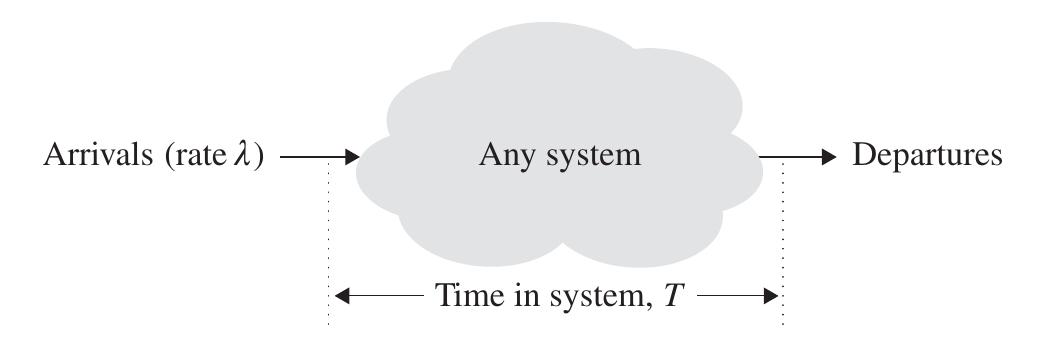
\includegraphics[scale=0.2]{images/setup_for_little_law.jpeg}
\caption{Setup for Little’s Law}
\end{figure}

\end{itemize}
	
\end{frame}


\begin{frame}
\frametitle{Little’s Law}
\framesubtitle{\textbf{\textit{Little’s Law for Closed Systems}}}

\begin{itemize}
\item \textbf{Little’s Law for Closed Systems}: For any ergodic closed system
$$N= X \cdot E [T ]$$
Here, 

$N$ = multiprogramming level 

$X$= throughput (the rate of job completions for the system)

$E [T ]$ =  mean time jobs spend in the system 


\begin{figure}
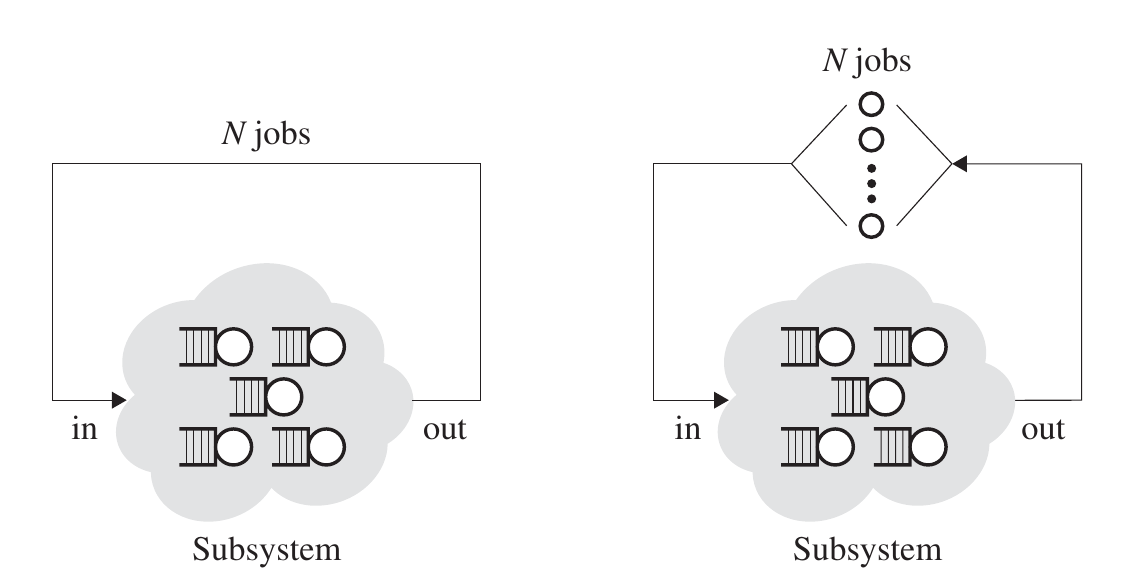
\includegraphics[scale=0.19]{images/little_law_for_closed_systems.jpeg}
\caption{ Little’s Law closed systems}
\end{figure}

\end{itemize}
	
\end{frame}


\begin{frame}
\frametitle{Restating Little`s Law Using Time Average}
\framesubtitle{\textbf{\textit{Little`s Law Proof's are in Book}}}
\begin{itemize}
\item From Chapter 5 

\begin{itemize}
\item 
$$\lambda = {\lim}_{t \rightarrow \infty } \frac{A(t)}{t} \:, 
\: X = {\lim}_{t \rightarrow \infty } \frac{C(t)}{t} $$
\item $A(t)$ = number of arrivals by time $t$ 
\item $C(t)$ is the number of system completions (departures) by time $t$
\end{itemize}

\item \textbf{Little’s Law for Open Systems Restated} : Given any system where
$ \overline{N}^{Time Avg}$ , $ \overline{T}^{Time Avg}$, $\lambda$, $X$
exist and where $\lambda = X$, 
$$ \overline{N}^{Time Avg} = \lambda \overline{T}^{Time Avg} $$

\item \textbf{Little’s Law for Closed Systems Restated} : For closed
system (interactive or batch) with multiprogramming level $N$ \&  given that $ \overline{T}^{Time Avg}$,  $X$ exists \&  $\lambda = X$, 
$$ N  = X \cdot \overline{T}^{Time Avg} $$

\end{itemize}
	
\end{frame}

%===============================
\section{ The Forced Flow Law}

\begin{frame}
\frametitle{ The Forced Flow Law}
\framesubtitle{\textbf{\textit{}}}
\begin{itemize}
\item The Forced Flow Law relates \textbf{system throughput} to the \textbf{throughput of an individual device} as follows:
$$X_i = E[V_i] \cdot X$$
Where,  $X$ = system throughput, $X_i$ = throughput at device $i$,
$V_i$ = number of visits to device $i$ per job = Visit ratio for device $i$.

\item Example : page 108

\end{itemize}
	
\end{frame}


\section{  Bottleneck Law}

\begin{frame}
\frametitle{  Bottleneck Law}
\framesubtitle{\textbf{\textit{}}}
\begin{itemize}
\item Let, $D_i$ =  total service demand on device $i$ for all visits of a single job (i.e., a single interaction). That is,
$$D_i = {{\sum}_{j=1}}^{V_i} {S_i}^{(j)}$$
${S_i}^{(j)}$ = service time required by the $j$ th visit of the job to server $i$
\item  assuming that the number of visits a job makes to device i is not affected by its service demand at the device.
$$E [D_i ] = E [V_i ] \cdot E [S_i ]$$

\item \textbf{Bottleneck Law} 
$$ {\rho}_i = X \cdot E[D_i] $$

\item  \textbf{Explanation}: $X$ jobs/sec arriving into system. Each  arrivals
into the system contributes $E [D_i ]$ seconds of work for device $i$. So device i is busy for $X \cdot E [D_i ]$ seconds out of every second (e.g., device i might be busy for half a second
out of every second). 

Thus $X \cdot E [D_i ]$ represents the utilization of device i.



\end{itemize}
	
\end{frame}
    
\end{document}